\documentclass{article}
\usepackage{nips07submit_e,times}
\usepackage{multirow}
\usepackage{graphics}
\usepackage{graphicx}


%\documentstyle[nips07submit_09,times]{article}


\title{Technical Report:\\ME Algorithm for Hierachical Dirichilet Process and Its Extensions}


\author{}



\newcommand{\fix}{\marginpar{FIX}}
\newcommand{\new}{\marginpar{NEW}}

\begin{document}
Donglai Wei and Erik Sudderth \\
Department of Computer Science\\
Brown University\\
Providence, RI 02912 \\
\texttt{\{donglai\_wei,sudderth\}@cs.brown.edu} \\

\makeanontitle

\begin{abstract}We here develop a Maximize-Expectation(ME) learning algorithm for Hierarchical Dirichilet Process(HDP)
and its extension Hierarchical Pitman-Yor Process(HPY).
We first show the advantage of ME algorithm over other varitional methods to learn Dirichlet Process Mixture model(DPM) as a baseline. 
Then we use Chinese Restaurant Franchise(CRF) representation to construct ME algorithm for HDP and test it on synthetic data. 
Later, we extend the ME algorithm to learn Hierarchical Pitman-Yor Process(HPY) model, which generalizes HDP with more flexiblility. 
Implementing our novel learning method, hopefully we will improve the learning performance of HPY model for shared segmentation problem.

\end{abstract}

\section{BackGround}
\subsection{Generalized Dirichilet Process}
During clustering, we may not only want to separate observations into different groups but also wish these groups to share common features. 
For example, in document modeling, the aim is to cluster words within the documents into different topics. 
When clustering documents from NIPS in machine learning and  computer vision, 
we may wish to allow topics like \textquotedblleft graphical model \textquotedblright and \textquotedblleft optimization\textquotedblright to be shared among them. 
\\ \\
Hierarchical Dirichilet Process(HDP), which natually handles the problem above, was formally introduced into unsupervised learning in Teh at.el[2].
Figure 1 shows the graphical model for DP mixture and HDP. But due to the complexity, the extant learning methods developed for HDP are far from maturity.


\subsection{ME Algorithm}
Consider a probabilistic model P(x,w,$\alpha$),where x is observed random variable, w hidden variable and $\alpha$ hyperparameter.   
For the generative approach to clustering, hidden variables are divided into two classes: cluster assignment z and generative model parameters $\theta$.  
Then the joint probability factors into: P(x,z,$\theta,\alpha$)=P(x$|z,\theta,\alpha$)P($\theta|\alpha$)P(z$|\alpha$). 
So the only problem remains in learning the distribution q(w) of hidden variable w.
For variational methods, the goal is to minimize the KL divergence between q(z,$\theta$) and the posterior distribution $p(w |\vec x,\alpha)$, which 
is equivalent to maximizing the lower bound for the likelihood:
\begin{eqnarray*}
log p(\vec x |\alpha)
&\geq&log p(\vec x | \alpha)-KL[q(\theta,\vec z) || p(\theta,\vec z | \vec x,\alpha)] \\
&=&-\boldmath{E}[log p(\vec x,\vec z, \theta | \alpha)]_{q(\theta,\vec z)}-H[q(\theta,\vec z)] 
\end{eqnarray*}
where $H(q(w))=-\int_w \ q(w)log [q(w)] dw$ is the entrophy.
Instead of estimating the joint distribution q(z,$\theta$), we factorize it into q(z)q($\theta$) which can be updated iteratively as coordinate ascent. 
In general, we can either maintains distribution estimation(known as E-step) or point estimation(known as M-step) for the hidden variable.
The popular Meanfield method iteratively estimates the disribution for z and $\theta$ with the following formula(also known as E-step).
\begin{center}
$q (\theta ) \propto exp(E[log P(\theta, z, D)]_{q(z)} ) \longleftrightarrow q (z) \propto  exp(E[log P(\theta, z, D)]_{q (\theta )})$.
\end{center}
In contrast, Kmeans algorithm keeps a point estimation for both $\theta$ and z. 
Discussed in [4], we can have four combinations of E-step and M-step for z and $\theta$. 
For our interest, we find ME algorithm(M-step for z, E-step for $\theta$) particularly fit the clustering problem for the following reasons:
1)In pratice, people may just want the optimal solution for the cluster assignment z instead of the real distribution of q(z).
2)For most of the timeAlso, the cluster assignment variable z is discrete and high dimensional, which makes the update formula hard to compute. 
So instead of maintaining the huge matrix for q(z), we may just pick out the MAP estimator(M-step) for q(z).
Since we don't want to be too greedy to also take M-step for q($\theta$), we end up with ME algorithm.

As discussed in [8],the goal of learning Generalized DP is to find the MAP estimation of the cluster
In the next section, we are going to show the advantage of ME algorithm for learning DP mixture model.

\section{ME Algorithm for HDP}  
Since the E-step for $\theta$ is trivial, the key of ME learning algorithm lies in the optimization problem of searching cluster assignment z.
\subsection{Formula}
For DPM with Gaussian conjugated with Normal-Inverse-Wishart distribution, Below is the derivation from [4].\\ \\ 
\emph{Likelihood Term}:$\ \ \ \ \ \ \ \ \ p(x_{n},\theta|\lambda,z_{n})=\mathcal{N}(x_{n}|z_{n},\mu,\Omega)
\mathcal{N}(\mu|m_{0},\xi_{0}\Omega)\mathcal{W}(\Omega|\eta_{0},B_{0})$\\ 
\emph{Label Term}: $\ \ \ \ \ \ \ \ \ \ \ \ \ \ \ p(\vec z|\lambda)=\frac{\Gamma(\phi_{0})}{\Gamma(N+\phi_{0})}\Pi_{k=1}^{K}\Gamma(N_{k}) \phi_{0}^{K}$\\
\emph{Object Function}: $log(p(x,z|\lambda))=log(p(x|z,\lambda))+log(p(z|\lambda))=$\\
(Likelihood)$ -\sum_{k=1}^{K} [\frac{D n_{..k}}{2}log\pi+\frac{D}{2}log\frac{\xi_{k}}{\xi_{0}}+\frac{\eta_{k}}{2}log det(B_{k})-\frac{\eta_{0}}{2}log det(B_{0})
-log \frac{\Gamma_{D}(\frac{\eta_{k}}{2})}{\Gamma_{D}(\frac{\eta_{0}}{2})}]$
\\
+
\\
(Label:)$log(\frac{\Gamma(\phi_{0})}{\Gamma(N+\phi_{0})})+\sum_{k=1}^{K}[log \Gamma(N_{k})+log\phi_{0}]$\\ \\
For HDP, we only need to change Label term. Here we use the Chinese Restaurant Franchise Representation.\\
Notation: J Restaurants, K global dishes, T tables, N datas,\\
$t_{ji}:$ the table that customer i in Restaurant j sits;\\
$k_{jt}:$ the dish that table t in Restaurant j serves;\\
$m_{jk}:$ number of tables in Restaurant j serving dish k;\\
$m_{.k}:$ number of tables serving dish k;\\
$m_{j.}:$ number of tables in Restaurant j;\\
$m_{..}:$ number of tables;\\
$n_{jtk}:$ number of customers in Restaurant j at table t eating dish k;\\
$n_{jt.}:$ number of customers in Restaurant j at table t;\\
$n_{j..}:$ number of customers in Restaurant j;\\
$p(k_{jt}|\vec k_{1},...\vec k_{j-1},k_{j1},...,k_{j(t-1)},\gamma)=\sum_{k=1}^{K}\frac{m_{.k}}{m_{..}-1+\gamma}\delta_{k_{jt}=k}+\frac{\gamma}{m_{..}-1+\gamma}\delta_{k_{ji}=\vec k}$\\ 
$p(t_{ji}|t_{j1},...,t_{j(i-1)},\alpha)=\sum_{t=1}^{m_{j.}}\frac{n_{jt.}}{i-1+\alpha}\delta_{t_{ji}=t}+\frac{\alpha}{i-1+\alpha}\delta_{t_{ji}=\vec t}$\\ 
$p(\vec z|\lambda)=p(\vec t,\vec k|\lambda)=\Pi_{j=1}^{J}[\frac{\Gamma(\alpha)}{\Gamma(n_{j..}+\alpha)}\Pi_{t=1}^{m_{j.}}(\Gamma(n_{jt.}))]\alpha^{\sum_{j=1}^{J}m_{j.}}
\times \frac{\Gamma(\gamma)}{\Gamma(T+\gamma)}\Pi_{k=1}^{K} [\Gamma(m_{.k})] \gamma^{K}$ \\ \\ \\
\subsection{Pseudocode}
We first try local search methods, corresponding to Posterior Gibbs Sampling in [7] and then add split\&merge approach. We randomized the algorithm
by randomly permute the order during searching.\\

{\bf Pseudocode:}\\
b$\sim$Uniform[0,1]\\
Switch (ceil(b*6)):\\
case 1: Local Search the best table for each customer\\
case 2: Local Search the best dish for each table\\
case 3: Split each table in each restaurant\\
case 4: Split each dish\\
case 5: Merge tables in each restaurant\\ 
case 6: Merge dishes\\
\section{Test Results}
We test Meanfield algorithm (EE) [1], Collapsed Meanfield algorithm(Collapsed EE)[5] and ME algorithm [3] implemented by Kurihara on the synthetic data, 200 random samples drawn from Gaussian of four mixtures.
We set almost same hyperparameters(except the one to generate mixture components) for these three algorithms and test with different initial cluster numbers.
Results are summarized in table 1. 
From figure 3 and 4, we can see that to some degree both EE and Collapsed EE suffer from local minimas and initialization.
Three variants of ME algorithms are tested here. Though the hierarchical clustering methods work perfect on this synthetic data, for real data top-down method uses heuristic criterion to split and merge while bottom-up method may have difficulty maintaining the huge distance matrix.
We here only try a naive local search. Though it does not perform well enough at first glance, it can be improved with advanced search algorithms and it fits best into Chinese Restaurant Franchise representation for Constructing HDP.
\begin{figure}[h] 
  \begin{minipage}[b]{0.5\textwidth} 
    \centering 
    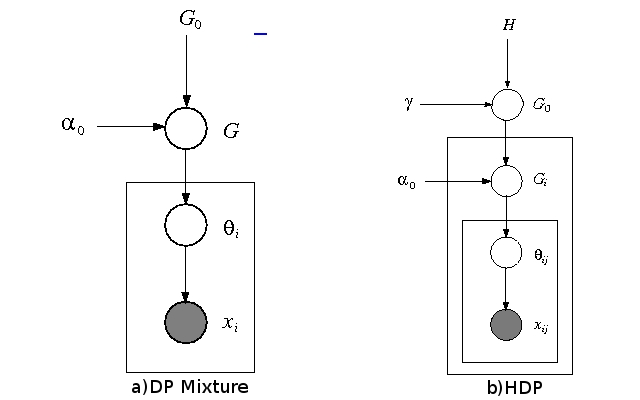
\includegraphics[width=0.8\textwidth]{dp.jpg} 
    \caption{Graphical Model for DP mixture and HDP} 
    \label{fig:by:table} 
  \end{minipage}% 
  \begin{minipage}[b]{0.5\textwidth} 
    \centering 
    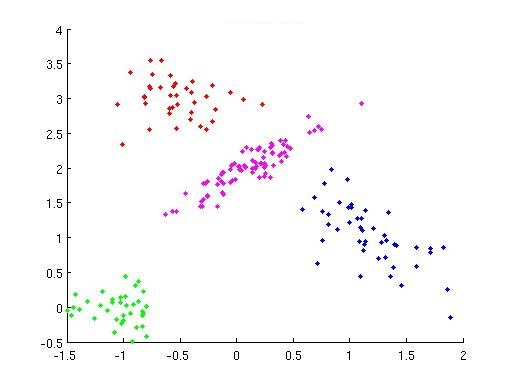
\includegraphics[width=0.8\textwidth]{truth.jpg} 
    \caption{Ground Truth 200 data from Gaussian Mixture} 
    \label{fig:by:table}  
   \end{minipage}% 
   \end{figure}
\begin{figure}[h] 
  \begin{minipage}[b]{0.5\textwidth} 
    \centering 
    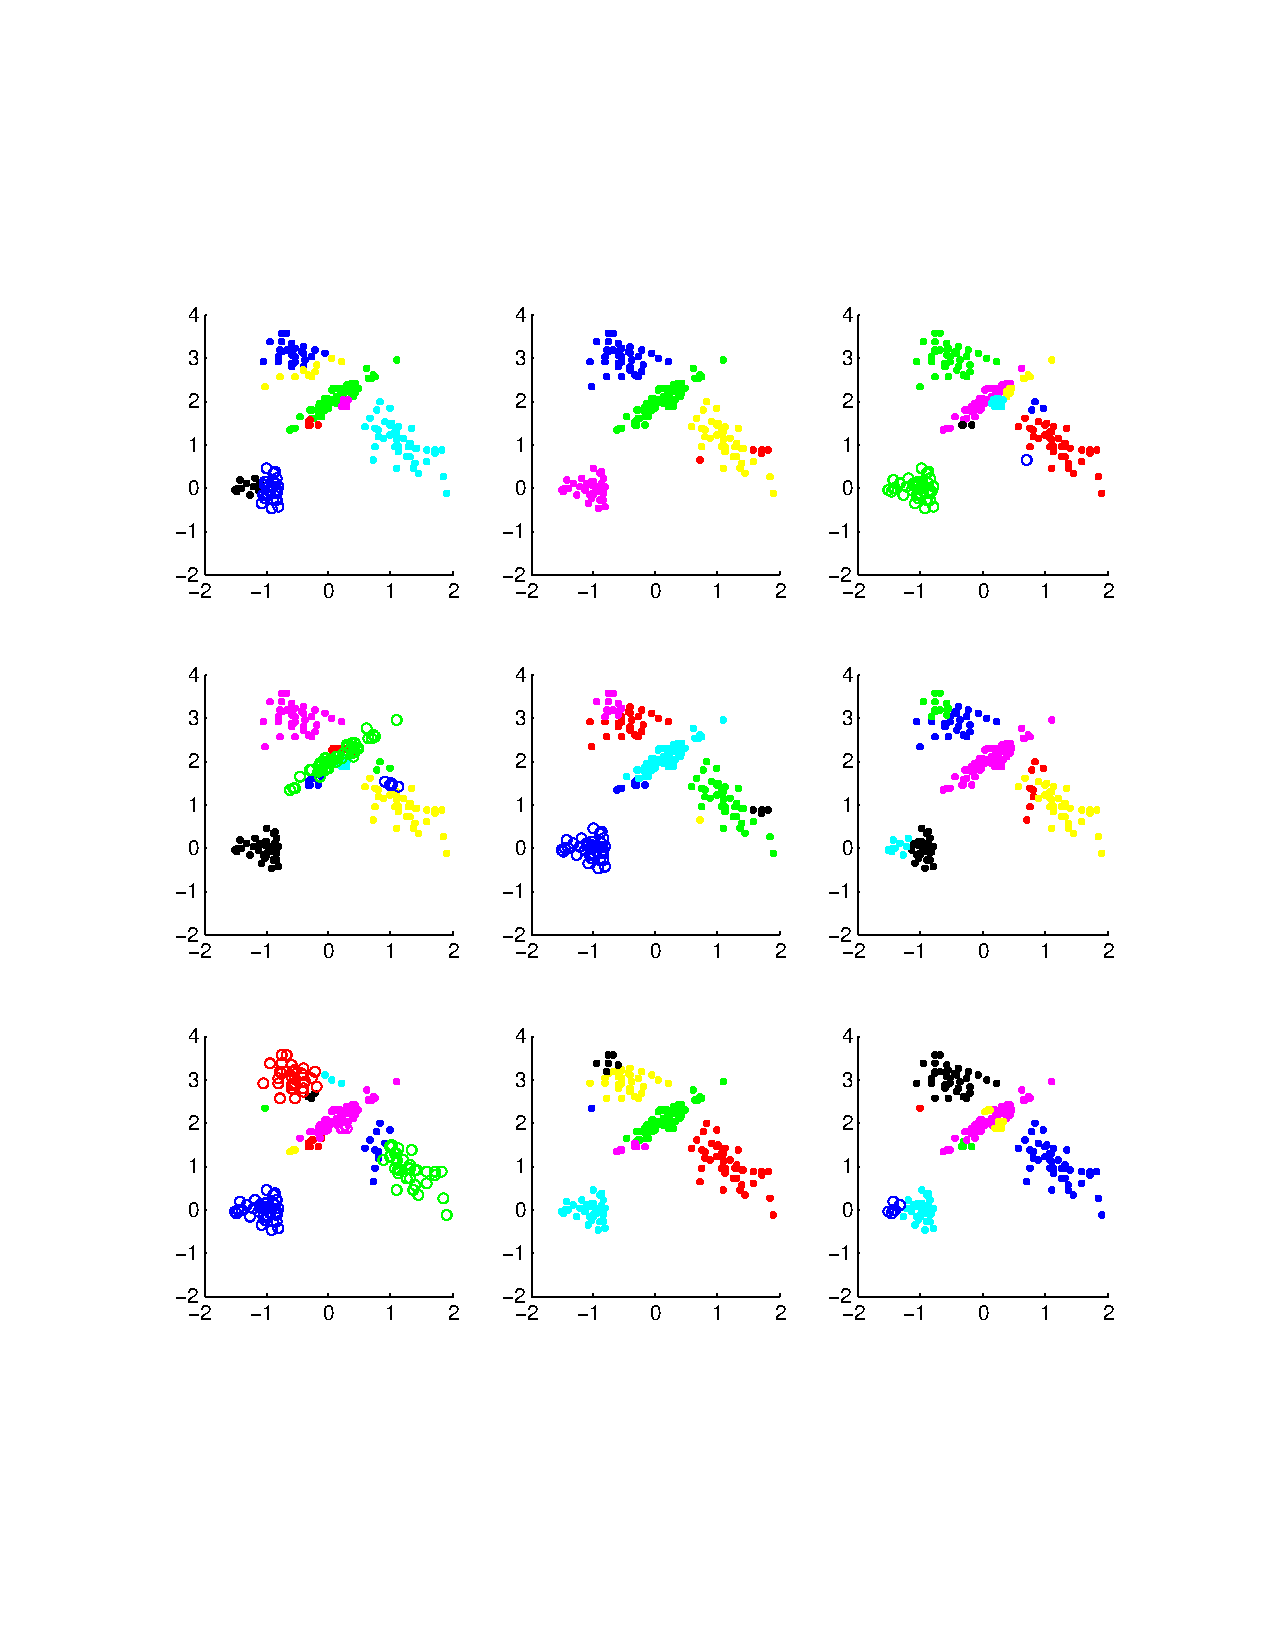
\includegraphics[width=0.8\textwidth]{BJ.pdf} 
    \caption{EE with random initialization, 20 inital clusters} 
    \label{fig:by:table} 
  \end{minipage}% 
  \begin{minipage}[b]{0.5\textwidth} 
    \centering 
    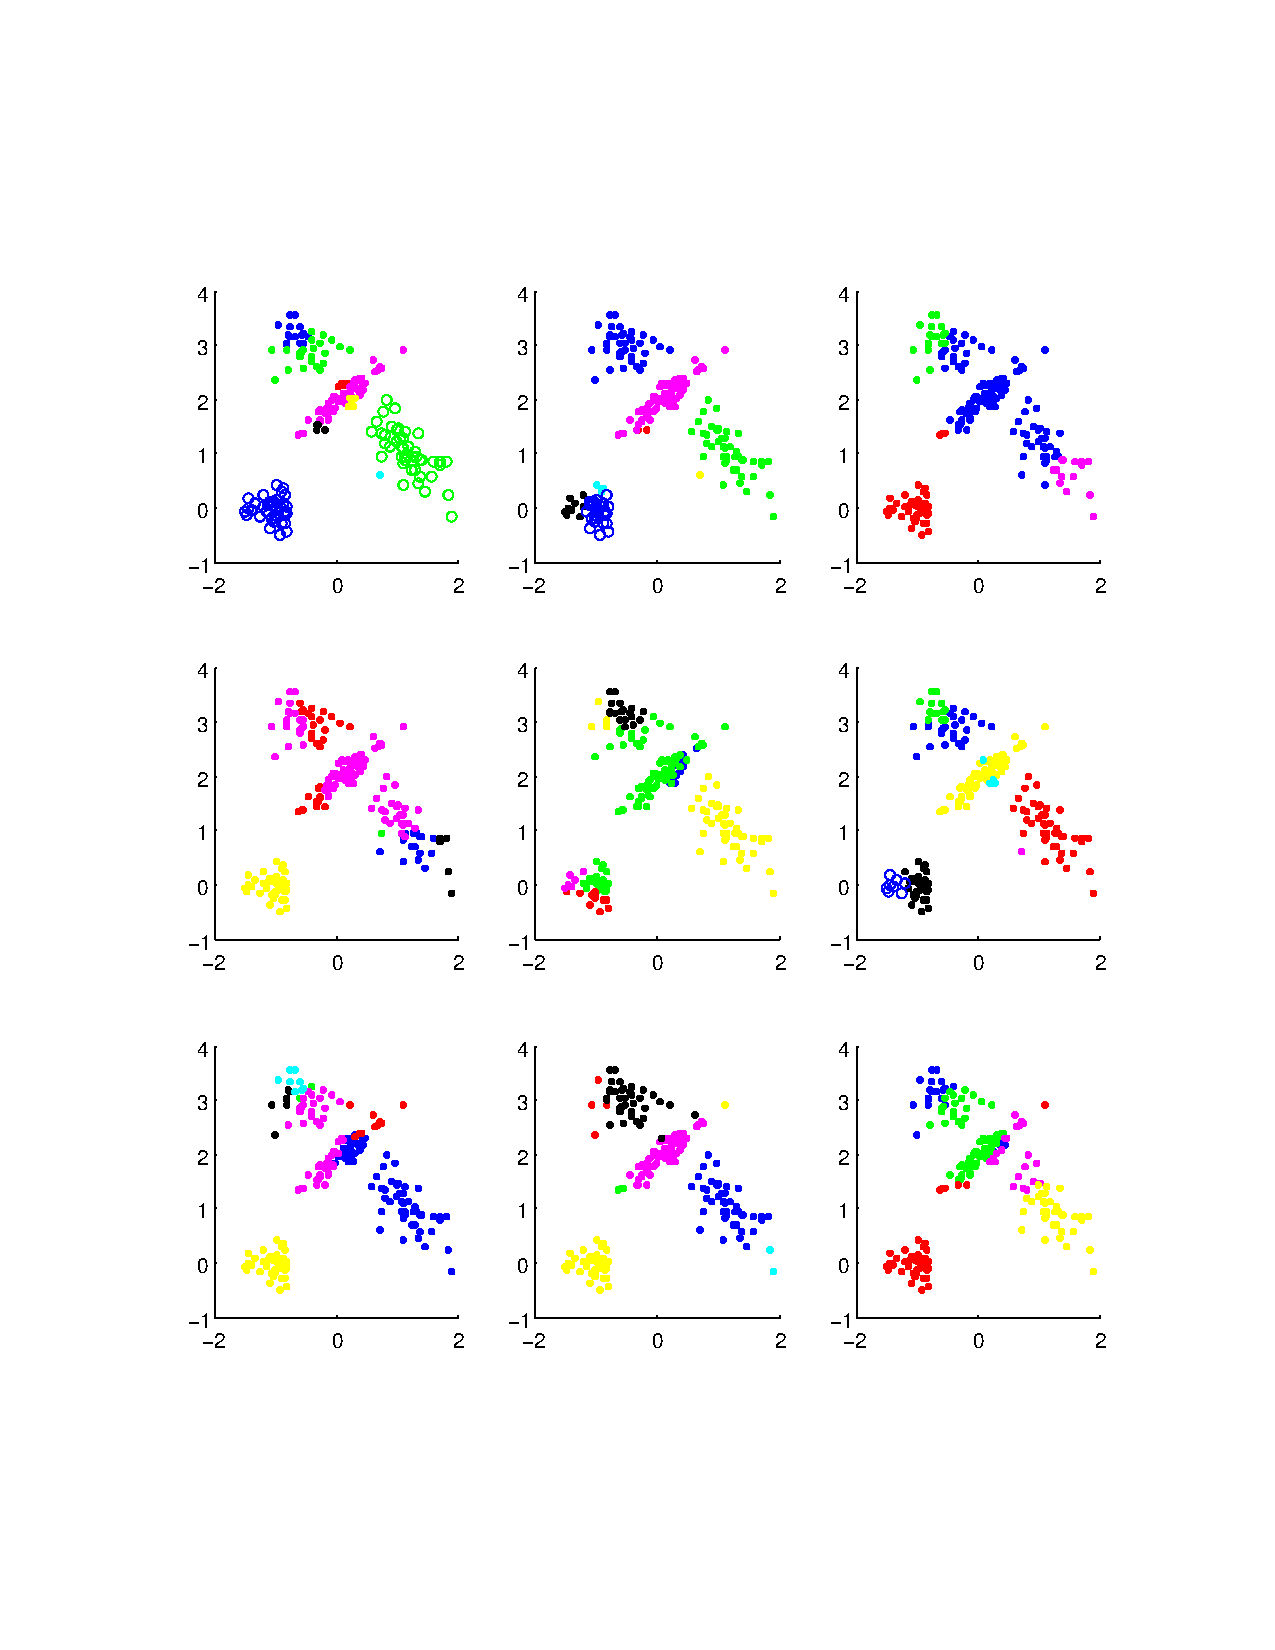
\includegraphics[width=0.8\textwidth]{cdb.pdf} 
    \caption{Collapsed EE with random initialization, 20 inital clusters}
    \label{fig:by:table}  
   \end{minipage}% 
   \end{figure}
\begin{table}[t]
\caption{Comparison of EE, Collapsed-EE and ME algorithms for DP mixture(with mean and std)}
\begin{center}
\begin{tabular}{|l|l|l|l|}

\hline
{\bf Learning Algorithm} &{\bf Initial Cluster Numbers} &{\bf Number of clusters}  &{\bf RandIndex} \\ 
\hline 
\multirow{2}{*}{EE(sampled initialization)} & 10 & 4.1(0.3) & 0.99(0.00) \\
					    & 20 & 4.1(0.3) & 0.99(0.00)\\
\hline
\multirow{2}{*}{EE(random initialization)}  & 10 & 6.9(1.2)&  0.97(0.01) \\
					    & 20 & 7.6(1.7)&  0.93(0.02) \\
\hline
\multirow{2}{*}{Collapsed EE}               & 10 & 5.6(1.6)&  0.90(0.22) \\
					    & 20 & 7.4(0.9)&  0.87(0.09) \\
\hline
\multirow{4}{*}{ME}                         & 1(Top-down) &    4  &  1 \\
					    & 200(Bottom-up) & 4  &  1 \\
					    & 200(Local search) & 15.5(3.9)&  0.83(0.09) \\
					    & 200(Local search+Merge) & 6.5(0.9)&  0.93(0.09) \\
\hline
\end{tabular}
\end{center}
\end{table}


\section{References}
\small{
[1]  Blei,D,M, Jordan,M.I, and Ng, A. Y. (2003), “Hierarchical Bayesian Models for Applications 
  in Information Retrieval,” in Bayesian Statistics, vol. 7, pp. 25–44 

[2] E.B.Sudderth and M.I.Jordan(2008)Shared Segmentation of Natural Scenes Using Dependent Pitman-Yor Processes NIPS 2008


[3] Ghahramani, Z. and Beal, M. J. (2000). Variational inference for Bayesian mixtures of                                                          ̈
  factor analysers. In S. A. Solla, T. K. Leen, \& K.-R. Muller (Eds.), Advances in neural
  information processing systems, 12. Cambridge, MA: MIT Press.

[4] K. Kurihara and M. Welling. Bayesian K-means as a
 ”maximization-expectation” algorithm. Neural Computation, 2008

[5] Y. W. Teh, K. Kurihara and M. Welling. Collapsed Variational Inference for HDP
NIPS 2007

[6] Y. W. Teh and M.I.Jordan.Hierarchical Bayesian Nonparametric Models with Applications.(2010) Bayesian 
Nonparametrics in Practice, Cambridge, UK: Cambridge University Press.

[7] Y. W. Teh, M. I. Jordan, M. J. Beal, and D. M. Blei. Hierarchical Dirichlet processes. Journal of the 
American Statistical Association, 101(476):1566–1581, 2006.

[8] Hal Daume ́III Fast search for Dirichlet process mixture models. UAI 2006
}


\end{document}
